\chapter{采样、强化学习与偏好优化}\label{采样与强化学习}

\section{解码与采样 多次尝试能发现什么}\label{解码与采样 多次尝试能发现什么}

我们修好 SFT 后，挑了一批稍难的题。模型第一次回答错了，我们再次问一次，相当于重新采样一次，却给出了有效解法。我们没有增加知识，只改变采样；这说明一次输出不能完整描述模型在该题上的行为分布。

有许多方法与采样结果有关。生成时，贪心解码（greedy decoding）每步选择最高概率 token，这样几乎每次推理的轨迹都是确定的，但这个唯一轨迹未必最优。随机采样（sampling）按概率抽取，可能产生许多不同思路的轨迹。温度通过缩放 logits 改变分布：温度较低通常更集中，较高通常更分散，但更分散不等于更多有效探索。核采样（nucleus sampling，也称 top-p sampling）只在累积概率达到阈值的候选中重新归一化采样，减少极低概率 token 的干扰。例如，在某一步 token 生成时，设置 top-p 为 0.9 的情况下，如果前三个 token 的累计概率已经达到了阈值，就只取这三个 token 进入采样，其他的大量 token 都忽略掉\footnote{top-k 类似，即选择前 k 个 token 重新计算概率分布然后采样。}。设前缀为 h、候选 token i 的 logit 为 z 的下标 i、正温度为 T，温度采样分布写为：
\[p_{T}(i \mid h) = \frac{\exp\left( z_{i}/T \right)}{\sum_{j}^{}\exp\left( z_{j}/T \right)}\quad\quad T > 0\]

这里 j 遍历词表候选，分母保证概率总和为 1。此处的 T 表示温度，与第 2.2 节表示序列长度的 T 不同；top-p 截断是在得到分布后进行的另一道处理。

我们用 pass@1 描述一次尝试的成功情况，用 pass@k 描述 k 次尝试至少有一次成功的情况。若每次独立且单次成功率相同为 p，那么至少一次成功的概率是 1 减去 k 次全部失败的概率。真实模型不同题的成功率不同，输出也可能高度重复，所以总体上不能随便把平均 p 当成准确评估。 在上述独立且等成功率的简化条件下，k 次中至少成功一次的概率写为：
\[P(at\ least\ one\ success) = 1 - (1 - p)^{k}\]

其中 p 是单次成功概率，k 是尝试次数；右边先计算全部失败的概率，再用 1 减去它。这是简化模型，不是对所有实际采样分布都成立的通用估计器。

最关键的区别是：pass@k 假设我们有办法识别哪次成功。它不等于系统最终只返回一个答案的正确率，只是一个期望值。数学题可以用答案验证器，代码可以用测试；开放式讲解往往还要人工或可靠评审。开放式问题人工审核在大部分情况下是无法实现的，所以我们通常只构造答案比较封闭的题目进行强化学习训练或者测评。

我们做一个题目难度画像。某些题几乎每次都对，某些题偶尔对，某些题在推理预算（即重试上限）内从未成功。中间那类题常适合从所有尝试中筛选正确的轨迹以或获得差异反馈，也就是用来指导参数优化方向；如果所有轨迹全错，表明这种题目对模型太难，需要进一步检查模型能力、格式和奖励；后面介绍 GRPO 时会看到：若只用同题组内的结果奖励构造相对优势，全错或全对的回答组缺少相对比较信号；PPO 的优势还依赖价值基线，不能直接套用这一结论。当然，有限次采样没成功，只能说明``在本次预算和采样配置下未见成功''，不能证明成功概率严格为零，有时候我们允许模型给出更多尝试。一个题目我们通常允许最少尝试 8 次，如果超过 32 次尝试都没有产生任何正确答案\footnote{这种情况下即便产生极少的正确答案，也有可能是 hack 来的，即存在猜测、作弊等行为，需要对过程做评判}，那么通常认为模型能力不足，需要回退到 SFT 增强相关知识。

我们现在有了一个连接训练与推理的观察：模型偶尔能走通的路径，可以变成后续训练的数据；而不同采样配置会改变哪些路径能被发现。接下来，我们先从最简单的筛选开始。

\textbf{本节相关资料}
\begin{enumerate}
    \item Chen 等，2021，\href{https://arxiv.org/abs/2107.03374}{Evaluating Large Language Models Trained on Code} 。阅读重点：pass@k 的定义及基于有限样本的估计方式。
    \item Wang 等，2022，\href{https://arxiv.org/abs/2203.11171}{Self-Consistency Improves Chain of Thought Reasoning in Language Models} 。阅读重点：采样与答案选择如何共同影响最终效果。
\end{enumerate}

\section{拒绝采样微调 RFT 把成功尝试变成示范}\label{拒绝采样微调 RFT 把成功尝试变成示范}

模型已经在部分难题上偶尔成功。我们让它对每题生成多个解答，再用验证器筛出正确结果，用这些结果继续做 SFT。这样，原来稀少的成功路径在下一轮更容易被生成。这就是本书所说的拒绝采样微调（Rejection Sampling Fine-Tuning，RFT）。

这个缩写在不同语境也可能表示 reinforcement fine-tuning。我们阅读论文时必须展开全称，避免把筛选后最大似然与强化学习混成同一种算法。此处的更新损失仍然是最大似然，改变的是训练数据的来源与筛选规则。

我们先用当前检查点采样，筛选后更新，再用新检查点重新生成。与当前策略分布一致的采样称为同策略（on-policy）采样\footnote{on-policy是传统强化学习常见的概念，简单来说，因为模型随着训练参数会一直变化，用最新的模型采样产生的策略/轨迹就是同策略，用旧的模型采样的策略就是异策略（off-policy），大模型领域绝大部分情况下都仅限同策略训练。}；筛选和后续参数更新又会改变这种对应关系。数据刚产生时接近当前策略分布，这样对模型的参数破坏性更小；经过筛选，它已经条件化到成功子集；随着参数更新，旧样本也逐渐变旧。因此，我们称它具有迭代的策略相关性，比简单贴上``完全 on-policy''更准确。若只在最初生成一次，以后反复训练，它就越来越像静态数据微调。

验证器是这条管线的关键。只检查最终答案，可能留下碰巧答对却推导错误的样本。代码通过公开测试，也可能不满足未覆盖的边界条件。我们不仅要筛对错，还要检查答案解析、等价形式、测试覆盖和数据泄漏。对于开放任务，也可以用奖励模型（通常是对齐人类偏好的模型，或者一个超强模型）或规则筛选，所以拒绝采样并非只适用于有唯一标准答案的任务；只是可靠筛选在可验证任务上通常更容易。

自学推理（Self-Taught Reasoner，STaR）让我们看到另一种办法：若模型直接解不出，可以在提供正确答案的条件下生成解释，再筛选有用的推理数据。这扩大了可获得示范的范围，也带来风险：知道答案以后写出的解释可能是事后合理化。我们需要检查解释本身，不能因为结论正确就默认过程正确。

RFT 的局限也逐渐清楚。比如成功样本可能集中在容易题和少数表达模式，非常单一；或者有些成功样本出现了 hack，只是答案正确，这种样本学了危害很大。需要注意的是，在工业界，一些团队为了确保模型在榜单上的分数，会非常大量采用 RFT 训练。虽然这些样本在榜单上能提高分数，但对模型的实际能力提升有限，甚至可能带来负面影响。因此，在使用 RFT 时，我们要注意样本的多样性和质量，避免过度依赖少数成功样本。

下一步的问题是：能否让不那么成功的尝试也参与比较，并让反馈直接改变策略？

\textbf{本节相关资料}
\begin{enumerate}
    \item Zelikman 等，2022，\href{https://arxiv.org/abs/2203.14465}{STaR Bootstrapping Reasoning With Reasoning} 。阅读重点：迭代自生成与 rationalization 如何产生新示范。
    \item Gulcehre 等，2023，\href{https://arxiv.org/abs/2308.08998}{Reinforced Self-Training ReST for Language Modeling} 。阅读重点：生成与改进如何迭代，以及筛选信号从何而来。
    \item Yuan 等，2023，\href{https://arxiv.org/abs/2308.01825}{Scaling Relationship on Learning Mathematical Reasoning with Large Language Models} 。阅读重点：采样成功与拒绝采样微调之间的联系。
\end{enumerate}

\section{人类反馈强化学习 RLHF 从偏好到策略更新}\label{人类反馈强化学习 RLHF 从偏好到策略更新}

现在，模型能给出两份都算对的解答。一份解释清楚，另一份跳过关键条件。二元答案验证器会给它们相同分数，但学生显然更需要前者。我们需要更细的目标：正确之外，还要有用、清楚、符合任务要求。

我们先收集偏好对，让标注者比较同一问题的两个回答。奖励模型（Reward Model，RM）学习一个分数，希望被偏好的回答通常得分更高。常见的 Bradley--Terry（布拉德利与特里）模型把两个奖励分数之差送入 logistic sigmoid（逻辑 S 形函数），得到偏好概率。这个分数只是从数据里拟合出的代理目标，不是``人类价值''的完整测量。 把问题记为 x、被偏好与不被偏好的回答分别记为 y 的上标加号与减号，偏好概率写为：
\[P\left( y^{+} \succ y^{-} \mid x \right) = \sigma\left( r\left( x,y^{+} \right) - r\left( x,y^{-} \right) \right)\]

符号``优于''表示偏好而非严格事实正确，r 是打分函数，σ 是把分数映射到 0 到 1 的 logistic sigmoid 函数。这里用来训练 RM 的是偏好标签。

有了奖励，我们把语言模型当作策略。状态是问题与此前生成的 token，动作是下一个 token，一段回答是一条轨迹。最简单的策略梯度直觉是：提高回报较高轨迹的概率，降低相对较差轨迹的概率。优势函数衡量结果比基线好多少。

我们先把反馈学习画成一个循环：采样产生当前策略实际会写的回答，评分器提供反馈，优化器据此更新策略，下一轮样本也随策略变化。图 \ref{fig:反馈训练数据流} 将``谁生成、谁评分、谁更新''分开；具体优势估计与更新规则会因算法而异。

\begin{figure}[t]
    \centering
    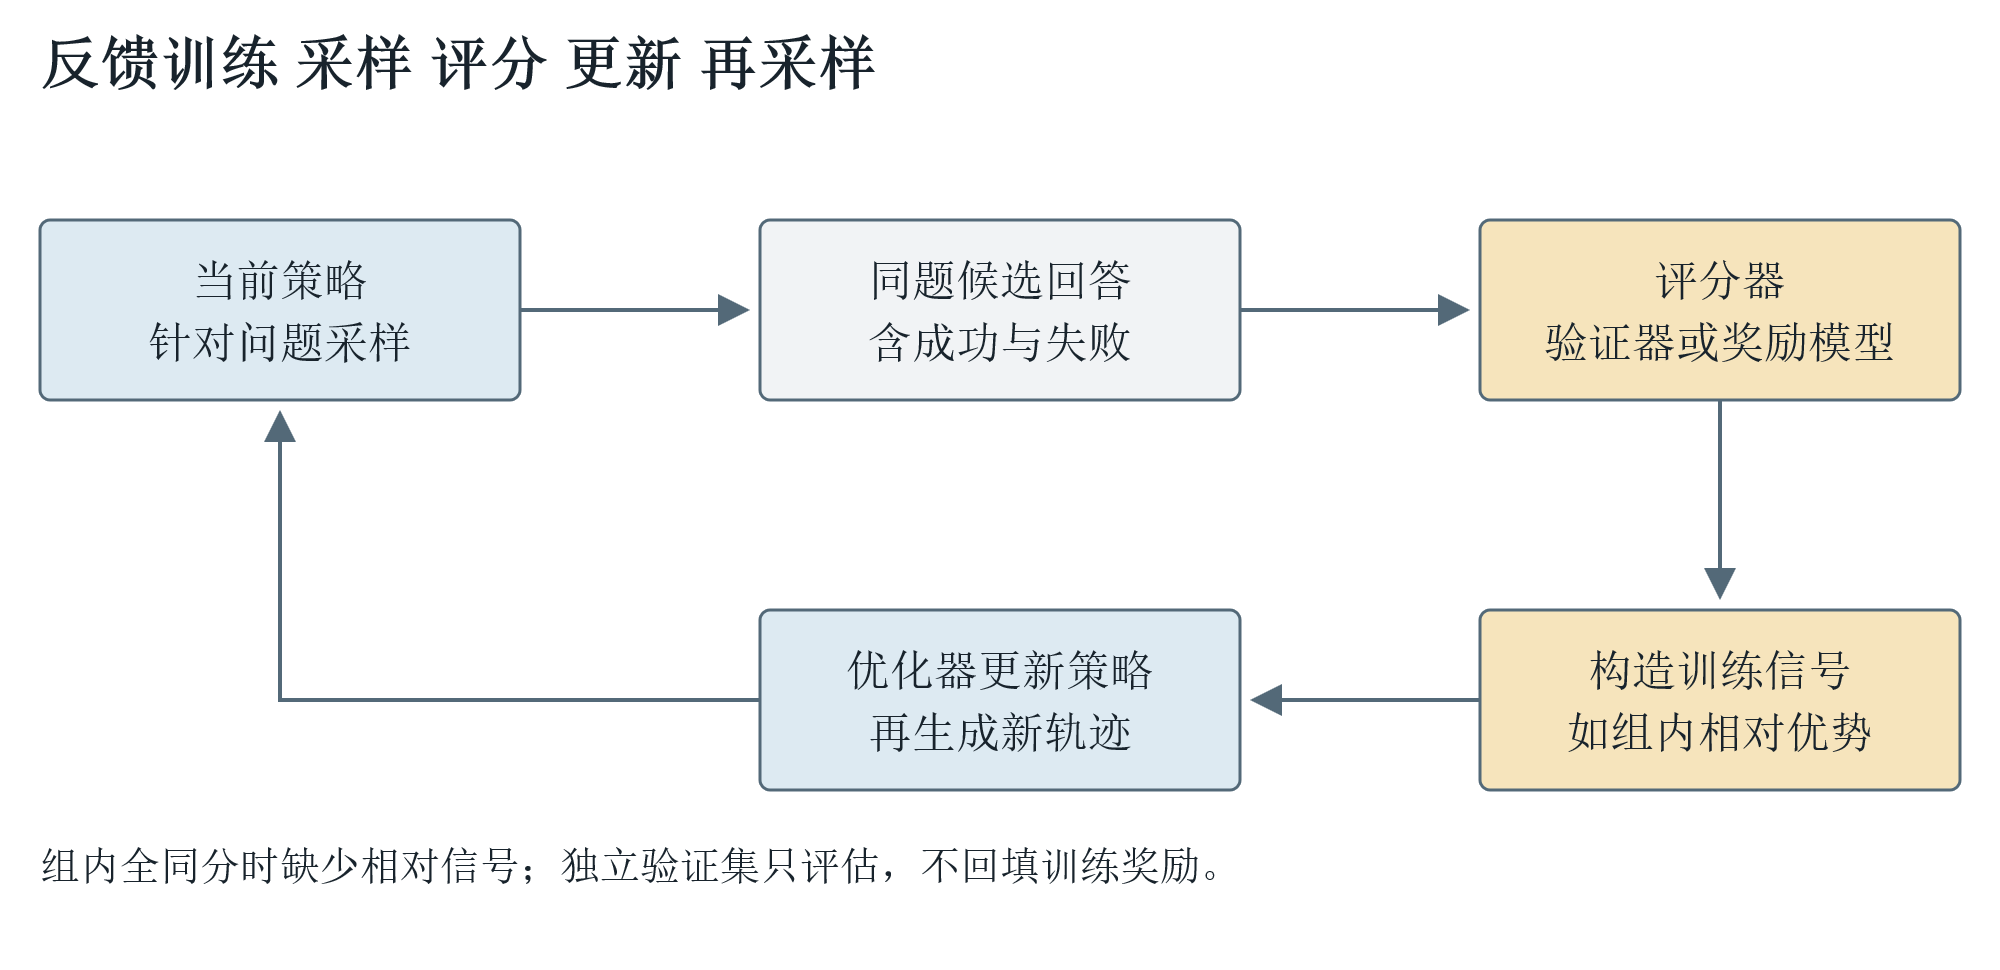
\includegraphics[width=\linewidth]{assets/media/image14.png}
    \caption{反馈训练的数据流。奖励模型与可执行验证器是两种不同评分来源；图中用组内相对优势作为后续分组比较算法的入口，不表示所有 RL 都必须采用分组比较。}
    \label{fig:反馈训练数据流}
\end{figure}

若只追求奖励最大，模型可能找到打分器的偏好捷径，例如冗长、讨好或固定套话。经典的人类反馈强化学习（Reinforcement Learning from Human Feedback，RLHF）因而常加入与参考策略的 KL 惩罚，控制偏离程度。KL 约束降低某些失控风险，却不保证真实质量；参考模型本身也可能有缺陷。 令 D 为训练问题分布、π 的下标 θ 为当前策略、π 的下标 ref 为固定参考策略，带 KL 正则且需要最大化的目标写为：
\[J(\theta) = E_{x \sim D,\, y \sim \pi_{\theta}( \cdot \mid x)}\left\lbrack r(x,y) \right\rbrack - \beta\, E_{x \sim D}D_{KL}\left( \pi_{\theta}( \cdot \mid x)\|\pi_{ref}( \cdot \mid x) \right)\]

期望符号表示对问题与生成回答求平均；第一项提高奖励，第二项扣除偏离参考策略的代价，β 是正的权衡系数。实际使用的是从采样估计的目标与梯度。

\textbf{近端策略优化（Proximal Policy Optimization，PPO）是一类策略优化方法。}本节重点介绍常见的 PPO-Clip：先用模型生成一批回答，再根据奖励估计每个生成位置的优势，最后在限制更新冲动的条件下，多次利用这批回答更新模型。``近端''可以先直观理解为：从已经采样验证过的策略附近出发，小步调整，再重新采样，这样确保参数更新是稳健的而非破坏性的。由于 PPO 算法非常重要，下面详细介绍。由于本材料尚未准备清晰的图示，强烈建议读者参考学习\href{https://datawhalechina.github.io/easy-rl/#/chapter5/chapter5}{蘑菇书}\footnote{https://datawhalechina.github.io/easy-rl/\#/chapter5/chapter5}中对 PPO 的更详细推导和图解，这也是笔者入门时的重要参考资料。

\subsection{把生成回答写成策略优化问题}

设问题为 $x$，模型生成的回答为 $y=(y_1,\ldots,y_N)$，$N$ 是本次回答的 token 数。在第 $t$ 步，状态和动作分别是：
\[
    s_t=(x,y_{<t}),\qquad a_t=y_t,\qquad
    \pi_\theta(a_t\mid s_t)=p_\theta(y_t\mid x,y_{<t}).
\]
状态就是``题目加上已经写出的内容''，动作就是下一个 token。$\theta$ 表示正在训练的语言模型参数。一次完整回答的概率是各步条件概率的乘积，取对数后则变成求和：
\[
    \pi_\theta(y\mid x)=\prod_{t=1}^{N}\pi_\theta(a_t\mid s_t),
    \qquad
    \log\pi_\theta(y\mid x)=\sum_{t=1}^{N}\log\pi_\theta(a_t\mid s_t).
\]
这说明提高某段回答的概率，最终要通过改变各个生成位置的条件概率来实现。我们不需要对``采样出一个离散 token''这个操作求导，而是在采样完成后，把得到的 token 序列送回模型，计算它们的对数概率，再对这些可微的数值求导。

在不折扣后续奖励的简化情形下，策略梯度的常见估计形式为：
\[
    \widehat g
    =\widehat{\mathbb E}_{t}
    \left[\widehat A_t\nabla_\theta
    \log\pi_\theta(a_t\mid s_t)\right].
\]
这里 $\nabla_\theta$ 表示对模型参数求梯度，$\widehat{\mathbb E}_t$ 表示在采样得到的有效生成位置上求经验平均，$\widehat A_t$ 是该位置的优势估计。严格的序列回报目标可先写成对每条轨迹逐步求和、再对轨迹求平均；这里用 token 平均展示常见训练形式，变长回答采用不同平均方式会改变样本权重。实现时必须明确这个选择，并用掩码排除提示词和补齐位置。

暂时把优势看成一个已经算好的数。若它为正，梯度上升会推动这次采到的动作变得更可能；若它为负，则推动它变得更不可能。这里改变的是``在这个前缀下生成这个 token''的倾向，改变的是条件概率分布。同时，参数又是共享的，所以实际更新还会影响其他前缀，所以这种更新也不意味着给词表里的某个 token 单独加减分。

与 SFT 相比，这里的训练方向由模型自己采样后的反馈决定：SFT 提高给定示范的概率；PPO 则既可能提高一次尝试的概率，也可能降低它。问题是，什么叫``比预期更好''，以及我们应当提高或降低多少？

\subsection{从奖励到回报，再到优势}

先区分三个概念。奖励是评分器在某一步给出的反馈；回报是从当前位置往后能够得到的累计奖励；优势则把回报与该状态下的预期水平比较。用 $\rho_t$ 表示逐步奖励，可以写成：
\[
    G_t=\sum_{j=t}^{N}\gamma^{j-t}\rho_j,
    \qquad 0\leq\gamma\leq 1.
\]
$G_t$ 是从第 $t$ 步起的采样回报，$\gamma$ 是折扣因子，越小越看重近期奖励。对于长度有限、主要关心最终回答质量的语言任务，可以取 $\gamma=1$。

最简单的结果奖励可以在回答结束时给出：中间各步 $\rho_t=0$，最后一步 $\rho_N=r(x,y)$。这并不意味着中间 token 没有训练信号：最终奖励会进入前面位置的回报。但是，只有最终结果时，算法很难精确知道哪一步推理真正起了作用；统计上加强一条高回报轨迹，也不代表这条轨迹里的每一步都已被证明正确。在大模型训练中尤其如此，对一个回答序列评判哪里推理得好哪里坏是非常贵的（可能需要专家或者强模型判定），通常简化为如果最终答案是对的，那么相同的奖励分配给这个序列生成的全部 token。

前面的参考策略 KL 惩罚，也可以放进逐步奖励。为了说明一种常见做法，设 $\pi_{\mathrm{old}}$ 是采样本批回答的策略，$\pi_{\mathrm{ref}}$ 是固定参考策略，定义：
\[
    k_t=\log\frac{\pi_{\mathrm{old}}(a_t\mid s_t)}
                         {\pi_{\mathrm{ref}}(a_t\mid s_t)},
    \qquad
    \rho_t=-\beta k_t+\mathbf{1}_{\{t=N\}}\,r(x,y).
\]
$\mathbf{1}_{\{t=N\}}$ 在最后一个位置取 1，其余位置取 0。这样，任务奖励在结尾加入，而偏离参考策略的代价沿回答累积。$k_t$ 是采样动作上的对数概率比，单次取值可以为负；只有对旧策略的动作分布取期望，才得到非负的条件 KL 散度。它不是每个 token 都必然为正的``距离''。这是在采样策略处估计 KL 惩罚的一种方式，具体系统也可以采用其他估计或直接正则化。

直接用回报更新，容易受到题目难度和奖励波动影响。价值模型（value model，也称 critic）因此学习 $V_\phi(s_t)$：在这个前缀下，按照相应策略继续生成，预期还能获得多少累计奖励。$\phi$ 是价值模型的参数。一个直观的优势估计是：
\[
    \widehat A_t=G_t-V_{\phi_{\mathrm{old}}}(s_t).
\]
$V_{\phi_{\mathrm{old}}}$ 表示更新前用来估计基线的价值模型。若实际回报是 1，而模型原来预计只有 0.4，优势就是 $0.6$，这次尝试比预期好；若回报是 0，而原来预计有 0.4，优势就是 $-0.4$。因此，奖励为正不保证优势为正，奖励为零也不保证没有梯度：关键是相对于什么预期来比较。

减去基线的作用，是减少策略梯度的波动。对于精确的、只依赖状态而不依赖当前动作的基线，在对应策略的动作分布下，有：
\[
    \mathbb E_{a\sim\pi_\theta(\cdot\mid s)}
    \left[V(s)\nabla_\theta\log\pi_\theta(a\mid s)\right]
    =V(s)\nabla_\theta\sum_a\pi_\theta(a\mid s)=0.
\]
因为所有动作概率之和恒为 1，所以减去这样的基线不改变理想策略梯度的期望。实际训练还涉及价值估计误差和后续裁剪等技巧。

\subsection{GAE 怎样把结尾反馈传回前面的 token}

PPO 常用广义优势估计（Generalized Advantage Estimation，GAE），把价值模型的预测与实际奖励结合起来。先定义一步的时序差分残差：
\[
    \delta_t=\rho_t+\gamma V_{\phi_{\mathrm{old}}}(s_{t+1})
                         -V_{\phi_{\mathrm{old}}}(s_t).
\]
它比较两个数：原来对当前状态的价值预测，以及``这一步实际拿到的奖励，加上对下一状态的价值预测''。如果后者更大，就意味着这一步之后的情况比原来预计得好。正常结束时，终止状态 $s_{N+1}$ 的价值设为 0；如果只是因为采样长度上限而中断，是否需要保留下一状态的价值估计，要按任务实际情况处理。

GAE 再把后续残差加权累积：
\[
    \widehat A_t^{\mathrm{GAE}}
      =\sum_{l=0}^{N-t}(\gamma\lambda)^l\delta_{t+l},
      \qquad 0\leq\lambda\leq 1.
\]
$\lambda$ 控制我们向后看多远。取 $\lambda=0$ 时，只用当前一步残差，较依赖价值预测；取 $\lambda=1$，且轨迹完整结束时，求和会化成采样回报减去当前价值。中间取值折中了价值估计误差与长轨迹回报的波动。

来看一个只含三个生成位置的教学例子，并非真实句子的分词。设中间奖励为 0，末尾奖励为 1，$\gamma=1$，三个位置的旧价值预测依次为 $0.4,0.6,0.8$，终止价值为 0。于是：
\[
    \delta_1=0+0.6-0.4=0.2,\quad
    \delta_2=0+0.8-0.6=0.2,\quad
    \delta_3=1+0-0.8=0.2.
\]
若再取 $\lambda=1$，三个优势就是 $0.6,0.4,0.2$。结尾的成功反馈通过求和影响了前面的位置，而前缀越接近已被预计会成功的状态，结果带来的额外惊喜越小。

\subsection{概率比 为什么需要保存采样时的旧策略}

生成回答很贵，我们希望同一批轨迹能用于若干次小批量更新。但更新一次以后，当前模型就不再是生成这批回答的那个模型了，偏离了 on-policy 的目标。如果仍不加区分地反复强化旧样本，就可能让模型过度偏向这一批偶然采到的结果。所以 PPO 通过重要性采样的方法来缓解这一问题，使得稍微旧一点的策略的样本仍然可用。

PPO 保存每个采样动作在旧策略下的概率，并在更新时计算概率比。这里用 $q_t$ 表示它，避免与奖励函数 $r(x,y)$ 混淆：
\[
    q_t(\theta)
      =\frac{\pi_\theta(a_t\mid s_t)}
                   {\pi_{\mathrm{old}}(a_t\mid s_t)}
      =\exp\left(\log\pi_\theta(a_t\mid s_t)
                 -\log\pi_{\mathrm{old}}(a_t\mid s_t)\right).
\]
分子是当前正在优化的策略，分母是本批采样时的策略；在这一批数据的若干轮更新中，分母保持不变。更新开始时两者相同，所以 $q_t=1$。若同一个前缀下，采到的 token 原概率是 0.10，当前概率变成 0.12，那么 $q_t=1.2$；变成 0.08，则 $q_t=0.8$。

在固定状态上，这种比值具有重要性加权的含义：用旧动作分布采样，也能对新动作分布下的某些量做加权估计。不过，PPO 仍然使用旧策略访问到的前缀；这个单步比值没有把所有状态分布变化都完整校正。因此，下面的式子是局部的代理目标，不是对任意新策略真实长期回报的精确计算：
\[
    L^{\mathrm{ratio}}(\theta)
      =\widehat{\mathbb E}_{t}
        \left[q_t(\theta)\widehat A_t\right].
\]
在旧策略处，对概率比求导，会得到前面策略梯度中的对数概率梯度形式。问题在于，如果只最大化这个目标，正优势动作的概率可以被不断提高，负优势动作的概率也可能被过度压低。为了避免更新幅度过大导致训练崩溃，PPO-Clip 通过裁剪重要性比率的方式缓解这一问题。

\subsection{裁剪目标 只给适度改进继续加分}

PPO-Clip 最大化的核心目标是：
\[
\begin{split}
    L^{\mathrm{CLIP}}(\theta)
    =\widehat{\mathbb E}_{t}\Big[
       \min\big(&q_t(\theta)\widehat A_t,\\
       &\operatorname{clip}(q_t(\theta),1-\epsilon,1+\epsilon)
                          \widehat A_t\big)\Big].
\end{split}
\]
其中 $\epsilon>0$ 是裁剪幅度；为方便手算，下面取 $\epsilon=0.2$。$\operatorname{clip}(q,0.8,1.2)$ 把小于 0.8 的输入变为 0.8，大于 1.2 的输入变为 1.2，区间内保持原值。$\min$ 则从原始项与裁剪项中，取对优化而言更保守的那个。注意我们在\textbf{最大化}这个目标；如果代码使用梯度下降，就要对策略目标取负号。

为什么不能只保留裁剪后的那一项？因为我们希望停止奖励``沿正确方向改得过多''，同时仍然惩罚``沿错误方向越改越差''。把优势的正负分开看，含义就清楚了\footnote{建议参考\href{https://datawhalechina.github.io/easy-rl/\#/chapter5/chapter5?id=\_522\-\%e8\%bf\%91\%e7\%ab\%af\%e7\%ad\%96\%e7\%95\%a5\%e4\%bc\%98\%e5\%8c\%96\%e8\%a3\%81\%e5\%89\%aa}{蘑菇书}里面的图示}。

\textbf{正优势：值得增加概率，但不要靠无限增加同一动作来刷目标。}假设 $\widehat A_t=0.6$，旧概率为 0.10，当前概率升到 0.13，则 $q_t=1.3$。原始项是 $1.3\times0.6=0.78$，裁剪项是 $1.2\times0.6=0.72$，最终取 0.72。概率已经沿鼓励方向提高得较多，再提高也不会让这个样本的直接策略目标继续增加。反过来，若当前概率降到 0.07，$q_t=0.7$，目标会取 $0.7\times0.6=0.42$，而不是裁剪项 0.48：正优势动作被压低这种不利变化，仍会被目标反映出来。

\textbf{负优势：值得降低概率，但也不要一次压得太狠。}假设 $\widehat A_t=-0.4$，旧概率仍为 0.10，当前概率降到 0.07，则原始项是 $0.7\times(-0.4)=-0.28$，裁剪项是 $0.8\times(-0.4)=-0.32$，最终取更小的 $-0.32$。对于最大化目标而言，从 $-0.4$ 提高到 $-0.32$ 已是改进；继续把概率压低，不再获得这一项的额外收益。若概率反而升到 0.14，目标会取 $1.4\times(-0.4)=-0.56$，继续惩罚把较差动作变得更可能的方向。

在优势固定、只考察单个位置时，同一个目标也可以写成：
\[
    \ell_t(\theta)=
    \begin{cases}
      \widehat A_t\min(q_t(\theta),1+\epsilon),
          & \widehat A_t\geq 0,\\
      \widehat A_t\max(q_t(\theta),1-\epsilon),
          & \widehat A_t<0.
    \end{cases}
\]
这揭示了裁剪的方向性：正优势主要限制过大的概率提升，负优势主要限制过大的概率压低。它不是把任何方向的变化都一律抹平。

还要避免一个常见误解：裁剪的是目标中的概率比，\textbf{不是执行一个硬约束，保证所有概率比始终落在 $[0.8,1.2]$ 内}。多个位置共享参数，其他位置的梯度、价值损失或其他正则项，仍可能把某个位置推到区间之外。裁剪也不能保证奖励每轮上升。因此还需要监控新旧策略的 KL、概率比、学习率和更新轮数；有的实现会在偏离过大时提前结束本批更新。

\subsection{价值模型怎样训练，四种模型各管什么}

策略模型需要优势，优势又依赖价值估计，所以价值模型也要更新。一种常见的回报目标由 GAE 构造：
\[
    \widehat R_t=\widehat A_t^{\mathrm{GAE}}
                   +V_{\phi_{\mathrm{old}}}(s_t),
    \qquad
    L_V(\phi)=\frac12\widehat{\mathbb E}_t
                  \left[(V_\phi(s_t)-\widehat R_t)^2\right].
\]
$\widehat R_t$ 是这批数据中固定的训练目标，不是奖励模型给的原始分数。最小化平方误差，是让价值预测接近这批轨迹提供的回报估计。计算策略损失时，缓存的优势被当作常量，不通过它反向修改价值模型；训练价值模型时，回报目标也应停止梯度。否则，模型可能通过修改``评判自己的尺子''来降低损失，而不是按预定目标学习。

如果把策略与价值部分写进一个用于梯度下降的示意损失，可以写成：
\[
    L_{\mathrm{train}}=-L^{\mathrm{CLIP}}+c_V L_V-c_H H,
    \qquad c_V,c_H\geq0,
\]
这个示意损失用于最小化，各个符号的含义如下：
\begin{itemize}
    \item $L_{\mathrm{train}}$ 是策略与价值部分组合后的训练损失。策略参数记为 $\theta$，价值模型参数记为 $\phi$；组合损失可以写成 $L_{\mathrm{train}}(\theta,\phi)$。
    \item $L^{\mathrm{CLIP}}$ 是 PPO 的裁剪策略目标，利用新旧策略的动作概率比和优势估计，衡量策略更新是否加强了高优势动作、减弱了低优势动作。原本需要最大化 $L^{\mathrm{CLIP}}$，因此改用梯度下降时写成 $-L^{\mathrm{CLIP}}$。
    \item $L_V$ 是价值预测的平方误差损失，即价值模型预测 $V_\phi(s_t)$ 与固定回报目标 $\widehat R_t$ 之间的误差。$c_V\geq0$ 是价值损失的权重，控制价值误差在组合损失中的比重；$+c_VL_V$ 表示训练要降低价值预测误差。
    \item $H$ 是当前策略的平均熵，衡量动作概率分布的分散程度。$c_H\geq0$ 是熵奖励的权重；$-c_HH$ 表示在最小化组合损失时鼓励更高的策略熵，$c_H=0$ 表示不使用熵奖励。
\end{itemize}
策略熵具体计算为
\[
H(\theta)=\widehat{\mathbb E}_t\left[
-\sum_a\pi_\theta(a\mid s_t)\log\pi_\theta(a\mid s_t)
\right].
\]
这里，$t$ 表示本批轨迹中的有效生成位置；$s_t$ 是第 $t$ 步生成前的状态，在语言模型中包含问题与已经生成的回答前缀。$a$ 表示一个候选动作，在语言模型中就是候选的下一个 token；$\sum_a$ 对所有候选 token 求和，而不是只计算实际采样到的 token。$\pi_\theta(a\mid s_t)$ 是参数为 $\theta$ 的当前策略在状态 $s_t$ 下生成 token $a$ 的概率。$\log$ 是自然对数。$\widehat{\mathbb E}_t$ 表示按本批数据中的有效生成位置计算经验平均，补齐位置不参与平均；帽号表示用有限样本估计，不代表整个状态分布下的精确期望。

例如，如果下一步只有两个候选 token，概率各为 0.5，单个位置的熵为 $-2\times0.5\ln0.5=\ln2\approx0.693$；如果一个候选 token 的概率趋近于 1，另一个趋近于 0，熵就趋近于 0。因此，熵奖励鼓励保留一定的输出多样性，但高熵本身不代表回答正确。策略熵描述当前分布是否分散，参考策略 KL 描述当前分布与参考分布相差多少，两者不是同一个量。

熵项不是每个语言模型 PPO 实现都必须使用；价值裁剪、优势归一化等也属于需要另行说明的实现选择。前面若已把参考策略 KL 计入奖励，这个示意式就不再额外重复扣一次相同的 KL。

经典 RLHF 管线中的四种角色，现在可以逐一对应：
\begin{itemize}
    \item \textbf{策略模型（actor）}负责生成回答，并通过 PPO 改变生成概率。
    \item \textbf{奖励模型（RM）}对问题与完整回答评分，提供任务反馈；在这一轮策略训练中通常固定。它回答``这份回答得到多少分''。
    \item \textbf{价值模型（critic）}读取生成前缀，预测未来累计奖励，用来估计优势；它随训练更新。它回答``写到这里，接下来预计能得多少回报''，与 RM 的输入和目标都不同。
    \item \textbf{参考策略}通常是固定的 SFT 模型，提供 KL 惩罚的参照，帮助控制相对训练起点的偏离。
\end{itemize}

旧策略还承担第五种逻辑角色：它是本批数据的生成者，提供概率比的分母。它通常是每轮采样时从当前策略确定下来的快照，可以通过保存旧 log probability 等方式使用，并不意味着始终额外常驻一个完整模型。\textbf{旧策略管的是``本批更新走了多远''，参考策略管的是``相对固定起点偏了多远''。}第一轮两者可能相同，后面旧策略随采样轮次刷新，参考策略通常保持不变，所以 PPO 裁剪与参考策略 KL 不能互相替代。价值与策略也可以共享部分参数，四种角色不一定等于四套完全独立的模型副本。

\subsection{把一轮 PPO 训练连起来}

回到小助的方程题，一轮训练可以按以下顺序理解：
\begin{enumerate}
    \item \textbf{生成。}从问题集合抽取一批题，用当前策略生成回答，此时把它视为本轮旧策略。保存生成 token、有效位置掩码和旧策略对这些 token 的 log probability。
    \item \textbf{评分。}用 RM 或验证器计算任务奖励，用参考策略计算所需的 KL 信号，并取得更新前的价值预测。按预定规则构造逐步奖励，区分正常结束与长度截断。
    \item \textbf{估计优势。}从回答末尾往前计算回报或 GAE，固定本批优势与价值训练目标。此时才确定哪些位置相对预期值得加强或减弱。
    \item \textbf{更新。}把本批数据分成小批量，重新计算当前策略概率比，优化裁剪目标，同时训练价值模型。可以重复若干遍，但旧 log probability 和本批优势不会在每一步偷偷换成新值；策略偏离过大时应限制继续复用这批数据。
    \item \textbf{刷新。}用更新后的策略重新生成下一批回答，获得新的旧策略基准。持续检查独立任务质量、奖励、参考 KL、价值误差、截断率和输出重复，而不只看策略损失是否下降。
\end{enumerate}

采样配置也属于算法的一部分。前面介绍的温度与 top-p 会改变实际生成分布；如果采样时用了截断或温度变换，概率计算就必须与所声明的行为策略和训练目标相一致。不能一边用某个分布生成，一边把另一个分布的概率直接当作采样概率，却仍声称比值完成了相应的重要性校正。

最后，PPO 不要求同一道题一定同时出现成功和失败样本。即使这一批答案全错，只要回报与价值基线仍有差异，策略或价值模型也可能收到更新；但这不保证反馈足以指明正确解法。如果奖励始终相同，价值基线又准确匹配回报，基于这些回报的优势就可能接近零。下一节的 GRPO 用同题组内比较构造优势，``全对或全错时组内没有奖励差异''才是那种设置下更直接的问题。

如果任务能可靠验证，我们也可以直接用答案正确性或执行结果奖励，不必训练 RM。这通常称为可验证奖励强化学习（Reinforcement Learning with Verifiable Rewards，RLVR）。开放偏好和可验证任务都能使用强化学习；RL 也可以有过程奖励，并非天生只给结尾一次反馈。

\textbf{本节相关资料}
\begin{enumerate}
    \item Schulman 等，2017，\href{https://arxiv.org/abs/1707.06347}{Proximal Policy Optimization Algorithms} 。\textbf{PPO的开创性论文}。阅读重点：旧策略概率比、优势与裁剪分别解决什么问题。
    \item Schulman 等，2015，\href{https://arxiv.org/abs/1506.02438}{High-Dimensional Continuous Control Using Generalized Advantage Estimation}。阅读重点：时序差分残差如何构成 GAE，以及价值基线、偏差和方差之间的关系。
    \item Ziegler 等，2019，\href{https://arxiv.org/abs/1909.08593}{Fine-Tuning Language Models from Human Preferences}。阅读重点：如何把偏好奖励、参考策略约束与 PPO 接入语言模型训练。
\end{enumerate}

\section{组相对策略优化 GRPO 同题比较如何产生信号}\label{组相对策略优化 GRPO 同题比较如何产生信号}

2025 年，正当全世界都在疑惑 OpenAI 是如何给 GPT-o1 模型训练出高质量的推理链的时候，DeepSeek-R1 横空出世，结合他们早先提出的组相对策略优化（Group Relative Policy Optimization，GRPO），在数学推理任务上取得了显著进展。这个方法既大幅节约了计算资源，还能训练出非常完整的原生思维链，大幅提高模型能力。这一模型及其技术报告一时间震惊了全世界，下面我们结合 PPO 算法介绍 GRPO 算法。

前面提到， PPO 要训练价值模型，预测每个前缀后面还能得到多少回报。GRPO 换了一种取得比较基准的方式：对同一道题采样多份回答，直接用这一组回答的奖励作比较。它由 DeepSeekMath 提出，后续也用于 DeepSeek-R1 等推理模型工作。下面沿用前一节的符号，重点解释它相对于 PPO 改了什么。

\subsection{第一处改变 用同题组内比较替代价值模型}

在前面介绍的 PPO 中，我们根据逐步奖励和价值预测计算 GAE。用最简单的完整轨迹形式来概括，就是比较``实际回报''与``价值模型原来预计的回报''：
\[
    \widehat A_t^{\mathrm{PPO}}=G_t-V_{\phi_{\mathrm{old}}}(s_t).
\]
这里的基线来自一个需要学习的函数。它可以随前缀变化：同一道题刚开始写，以及已经完成关键推导时，对成功的预期并不一样。代价是要保存、运行和训练价值模型，而且价值估计不准也会影响优势。

GRPO 在常见的结果奖励设置中，不再预测每个前缀的价值。设同一个问题 $x$ 的 $G$ 份回答是 $y_1,\ldots,y_G$，由本轮旧策略采样得到，各自奖励为 $r_1,\ldots,r_G$。先计算组内均值和标准差：
\[
    \overline r=\frac1G\sum_{i=1}^{G}r_i,
    \qquad
    \sigma_r=\sqrt{\frac1G\sum_{i=1}^{G}(r_i-\overline r)^2}.
\]
再把第 $i$ 份回答的优势写为：
\[
    \widehat A_i=\frac{r_i-\overline r}{\sigma_r+\delta},
    \qquad \delta>0.
\]
这里明确采用除以 $G$ 的总体标准差，$\delta$ 是防止除零的小常数，与 PPO 裁剪幅度 $\epsilon$ 不同。直觉上，我们把``比模型原来预计的好多少''，换成``比同一道题的其他尝试好多少''。均值提供比较基准，除以标准差则对优势尺度做归一化。

例如四份回答的奖励是 $(0,1,1,0)$。均值为 $0.5$，标准差也为 $0.5$，忽略很小的 $\delta$ 后，优势约为：
\[
    (\widehat A_1,\widehat A_2,\widehat A_3,\widehat A_4)
      =(-1,1,1,-1).
\]
同一道题内，两份成功回答受到加强，两份失败回答受到抑制。我们只需要生成与评分，就能构造这组优势，因此省去了这里的价值模型、GAE 计算和价值损失。

\subsection{第二处改变 从逐位置优势变成整段回答的相对分数}

PPO 的 GAE 会结合各个前缀的价值预测，得到可能随位置变化的 $\widehat A_t$。对于这里只在结尾评分的 GRPO，同一份回答的所有有效生成位置使用同一个优势：
\[
    \widehat A_{i,t}=\widehat A_i,
    \qquad t=1,\ldots,N_i,
\]
其中 $N_i$ 是第 $i$ 份回答的长度。也就是说，只要这份回答比组内平均更好，它采到的各个 token 都沿着加强概率的方向参与更新；比组内平均更差，则沿相反方向参与。

这种做法简化了训练，却没有精确解决步骤归因。若一份答案碰巧猜对，错误推导也可能受到加强；若前半段正确、最后一步算错，前面的有效步骤也可能随整段回答受到抑制。因此，奖励是否可靠、是否需要过程检查，依然重要。这里讲的是结果监督（Outcome Reward Model，通常简称 ORM），因为；如果提供逐步奖励，GRPO 也可以构造随位置变化的优势，GRPO 本质上是通过组内差异确定优化方向，跟整段轨迹共用同一个奖励值没有必然联系。工业领域通常在答案可可靠验证的情况下用 ORM，这样成本最低。相对应的，如果要用过程监督（Process Reward Model，PRM）进行训练，GRPO 也可以在每个位置使用不同的奖励和优势，但 PRM 的尝试大多成本高且效果不佳。

\subsection{保留的部分 概率比与 PPO 裁剪仍然存在}

GRPO 并不是算完组内分数后，直接拿成功回答再做一次 SFT。它仍然计算当前策略相对采样旧策略的概率比：
\[
    q_{i,t}(\theta)=
    \frac{\pi_\theta(y_{i,t}\mid x,y_{i,<t})}
         {\pi_{\mathrm{old}}(y_{i,t}\mid x,y_{i,<t})}.
\]
这里比 PPO 多了一个回答编号 $i$，概率比本身的意义没有改变。把前一节的裁剪项记为：
\[
\begin{split}
    C_{i,t}(\theta)=\min\big(&q_{i,t}(\theta)\widehat A_i,\\
       &\operatorname{clip}(q_{i,t}(\theta),1-\epsilon,1+\epsilon)
                        \widehat A_i\big).
\end{split}
\]
正优势不再鼓励过大的概率提升，负优势不再鼓励过大的概率压低，含义与 PPO 相同。旧策略仍需在本批更新中固定，训练后也仍要用新策略重新采样。因此，GRPO 替换的关键是优势的来源。

\subsection{第三处改变 KL 可以单独放进优化目标}

在前一节展示的 PPO 实现里，参考策略的 KL 惩罚被折算进逐步奖励，再进入回报与 GAE。DeepSeekMath 原始 GRPO 的写法则把 KL 作为目标中的独立惩罚，使组内优势由任务奖励构造。

为把含义写清楚，我们先用每个前缀上的完整词表 KL 表示正则项：
\[
    K_{i,t}(\theta)=\sum_a\pi_\theta(a\mid s_{i,t})
       \log\frac{\pi_\theta(a\mid s_{i,t})}
                     {\pi_{\mathrm{ref}}(a\mid s_{i,t})},
    \qquad s_{i,t}=(x,y_{i,<t}).
\]
$a$ 遍历下一个 token 的候选。它比较的是当前策略与参考策略在同一个前缀上的动作分布，不是当前策略与旧策略的概率比。一个便于对照的 GRPO 目标写为：
\[
    J_{\mathrm{GRPO}}(\theta)=
      \mathbb E_{\substack{x\sim D,\\
                  y_{1:G}\sim\pi_{\mathrm{old}}(\cdot\mid x)}}
      \left[\frac1G\sum_{i=1}^{G}\frac1{N_i}
         \sum_{t=1}^{N_i}\left(C_{i,t}(\theta)-\beta K_{i,t}(\theta)\right)
      \right].
\]
外层期望表示对题目和旧策略生成的回答组求平均；$1/G$ 对回答求平均；$1/N_i$ 对一份回答内部的有效位置求平均。第一项根据组内优势和裁剪更新策略，第二项限制偏离参考策略。公式这里是完整词表 KL，实际上浪费了大量计算资源，因为绝大部分 token 的概率都几乎为 0，可以用 top-k 选择头 k 个 token 重新计算概率分布然后计算 KL 散度。$\beta$ 是 KL 惩罚系数，通常在训练中保持不变。

这种按回答再按长度平均的写法，让每份回答先形成一个平均贡献，而不是天然让长回答因 token 多而获得更大总权重。但不同的长度归一化会改变优化偏好，不能把长度处理当作无关紧要的细节。后续变体可能调整它、去掉组内标准差缩放，或者改变 KL 设置；GRPO 公认的改进包括 DAPO，GSPO 等，都是在这个基础上做的。

这里对比的是两种具体写法，并不是说 PPO 必须把 KL 放进奖励、GRPO 永远必须单独加 KL。无论采用哪种算法，旧策略仍然是采样与裁剪的基准，参考策略仍然提供偏离惩罚的参照。

\subsection{高熵 token 为什么值得重点训练}

前面的策略目标把每个有效生成位置都纳入更新。进一步的问题是：一段推理中的所有位置，对学会解题贡献是否相同？有些位置主要延续熟悉的词语与格式，有些位置则面对多种合理续写，选择之后会进入不同的推理路径。识别后面这类位置，可以帮助我们把训练信号集中到更有选择空间的决策点。

\textbf{高熵描述一个位置的候选分布}~在第 $i$ 份回答的第 $t$ 个生成位置，用采样时的旧策略计算熵：
\[
H_{i,t}=-\sum_{v\in\mathcal V}
\pi_{\mathrm{old}}(v\mid s_{i,t})
\log\pi_{\mathrm{old}}(v\mid s_{i,t}).
\]
这里，$i$ 是回答编号，$t$ 是回答中的生成位置，$s_{i,t}$ 是问题与此前已生成 token 构成的前缀，$\mathcal V$ 是词表，$v$ 遍历候选 token。$\pi_{\mathrm{old}}(v\mid s_{i,t})$ 是采样策略对候选 token 的条件概率，$\log$ 是自然对数，因此 $H_{i,t}$ 的单位为 nat。概率集中在少数候选上时，熵较低；多个候选都有较大概率时，熵较高。文献把高熵位置上生成的 token 简称为高熵 token，熵的计算对象是生成前的完整候选分布。

例如，假设某个位置只有两个候选，概率为 $(0.99,0.01)$，熵约为 0.056 nat；另一个位置的候选概率为 $(0.5,0.5)$，熵约为 0.693 nat。第二个位置有更大的选择空间。单个已采样 token 的惊讶度则是 $-\log\pi_{\mathrm{old}}(y_{i,t}\mid s_{i,t})$，其中 $y_{i,t}$ 是实际生成的 token。即使分布很集中，偶尔采到概率为 0.01 的候选也会得到较高惊讶度；按熵筛选时仍使用该位置的整个分布。

\textbf{为什么这些位置可能影响推理方向}~例如，模型写到``接下来采用''时，可以继续代入、分类讨论或反证，不同续写会改变后续求解过程；已经选定公式后，固定表达中的部分 token 则较容易预测。对于已经掌握基本语言与解题表达的模型，强化学习可以重点调整前一类选择：利用成功轨迹提高有效分支的概率，利用失败轨迹降低低收益分支的概率。熵提供候选位置，奖励与优势提供更新方向；正优势加强该位置实际采取的选择，负优势减弱该选择。

\textbf{怎样在损失里选择训练位置}~一种实现方式是根据采样批次中有效生成位置的熵确定阈值 $\tau$，保留熵最高的一部分位置，定义固定掩码
\[
m_{i,t}=\mathbf 1[H_{i,t}\geq\tau],\qquad
J_{\mathrm{select}}(\theta)=
\frac1G\sum_{i=1}^{G}\frac1{N_i}
\sum_{t=1}^{N_i}m_{i,t}C_{i,t}(\theta).
\]
这里，$m_{i,t}$ 是位置选择掩码，$\mathbf 1[\cdot]$ 在条件成立时取 1，否则取 0；$\tau$ 是熵阈值，例如按有效位置的熵分位数选取最高的 20\%。$G$ 是同题回答数，$N_i$ 是第 $i$ 份回答的有效生成长度，$C_{i,t}(\theta)$ 是前面定义的裁剪策略目标，$\theta$ 是当前策略参数。这个示意式沿用按完整回答长度归一化的方式，只展示策略更新项；KL 正则仍按具体训练配置单独组织。熵与掩码在本批更新中作为固定的选择依据，梯度通过保留位置的策略目标计算。

当 $m_{i,t}=0$ 时，该位置不直接贡献策略目标；整段回答仍参与生成，也作为后续位置的上下文。注意力连接使保留位置的梯度能够通过前缀计算传播，共享参数更新后，各个位置的输出分布也会随之改变。选择性训练因此减少了直接参与策略目标的位置，完整的采样与前向计算仍承担轨迹生成和熵统计的工作。

\textbf{实验支持了什么}~Wang 等人在 2025 年的《Beyond the 80/20 Rule》中研究了基于可验证奖励的强化学习（Reinforcement Learning with Verifiable Rewards，RLVR）。在其 Qwen3 推理训练实验中，仅保留熵最高的 20\% 位置的策略梯度，在 8B 模型上取得与全位置训练相当的表现，在 14B 和 32B 模型上取得更高表现；只训练熵最低的 80\% 位置则明显退化。论文报告，32B 模型在 AIME 2025 上相对全位置训练提高约 11.04 个百分点。这组对照支持把训练重点放在高熵决策位置的做法。

在训练诊断中，可以同时记录逐位置熵、选中比例和独立题集成绩，并比较全位置、高熵位置、低熵位置与随机位置四种更新方式。由此可以判断当前模型的收益来自哪些位置，选择合适的保留比例，并把策略更新集中到更有效的推理决策上。

\subsection{省下什么，又付出什么}

从训练流程看，原来的``采样、评分、预测价值、计算 GAE、更新策略与价值模型''，变成了``同题多次采样、评分、计算组内优势、更新策略''。价值模型的前向计算、反向传播及相应参数和优化器状态可以省去，但同一道题现在要生成多份回答。在固定总生成 token 预算下，分给一题的尝试越多，本批能够覆盖的不同题目就可能越少。PPO 也可以对同题多次采样，区别在于这里的组内比较直接依赖这些样本。

组内比较还带来一个明确限制。若四份回答全错，奖励都是 0，则组内均值是 0，标准差也是 0，加上 $\delta$ 后优势仍全为 0；若四份全对且奖励相同，优势也全为 0。这一组没有从结果奖励中产生相对策略信号，所以没有任何优化效果。相比之下，PPO 即使遇到相同奖励，也可以因为价值预测与回报不同而产生非零优势。

即使组内优势为零，独立 KL 正则也仍可能有梯度，所以不能说模型参数一定不变。若大量题目都产生零方差组，我们应检查题目是否过难或过易、奖励是否过于粗糙、采样是否缺乏差异。

标准差缩放也会影响题目之间的权重。例如四份回答只有一份成功，奖励为 $(0,0,0,1)$，均值为 $0.25$，标准差为 $\sqrt{3}/4$；忽略 $\delta$，唯一成功回答的优势约为 $1.73$，每份失败回答约为 $-0.58$。它们与两对两错时的 $\pm1$ 不同。可见，归一化不只是方便显示分数，也实际改变了各条轨迹的更新权重，仍需要结合题目分布评估。

回到小助，GRPO 的主要变化可以归结为：用同题的实际尝试构造比较基准，省去学习价值函数的环节，同时保留带裁剪的策略更新。我们因此除了看平均奖励，还要看每题成功率、零方差组比例、输出重复率、截断率和长度分布。只有这些信号一起改善或者保持，才能判断省下价值模型后，采样和比较是否仍在有效推动学习。

\textbf{本节相关资料}
\begin{enumerate}
    \item Shao 等，2024，\href{https://arxiv.org/abs/2402.03300}{DeepSeekMath Pushing the Limits of Mathematical Reasoning in Open Language Models}。阅读重点：第 4.1 节如何替换价值基线、保留裁剪目标，以及区分结果监督与过程监督的优势构造。
    \item DeepSeek-AI 等，2025，\href{https://arxiv.org/abs/2501.12948}{DeepSeek-R1 Incentivizing Reasoning Capability in LLMs via Reinforcement Learning}。阅读重点：GRPO 如何与奖励、冷启动及多阶段训练配合，避免把模型效果全部归因于单个算法。
    \item Wang 等，2025，\href{https://arxiv.org/abs/2506.01939}{Beyond the 80/20 Rule: High-Entropy Minority Tokens Drive Effective Reinforcement Learning for LLM Reasoning}。阅读重点：逐位置生成熵、高熵位置策略梯度掩码，以及与全位置和低熵位置训练的对照。
\end{enumerate}

\section{直接偏好优化 DPO 为什么可以绕过奖励模型}\label{直接偏好优化 DPO 为什么可以绕过奖励模型}

假如我们已经收集了``同一题，两份回答，哪份更好''的数据。PPO 路线先把它们变成奖励模型，再在线采样更新策略。我们自然会问：能否直接像对比学习一样用偏好对训练模型，少维护一个奖励模型？直接偏好优化（Direct Preference Optimization，DPO）就从这个问题进入，正如其论文名称所说：``你的大语言模型本身就是一个隐藏的奖励模型''。

\textbf{先读懂最优策略公式}~策略就是模型面对问题 \(x\) 时，对不同回答 \(y\) 分配的概率。参考策略 \(\pi_{ref}\) 是一份冻结的基准模型，通常取偏好训练开始前的 SFT 模型。先假设奖励 \(r(x,y)\) 已经给定，带 KL 正则的目标是：
\[
\max_{\pi}\;\mathbb{E}_{y\sim\pi(\cdot\mid x)}[r(x,y)]
-\beta D_{KL}\bigl(\pi(\cdot\mid x)\|\pi_{ref}(\cdot\mid x)\bigr),\qquad\beta>0.
\]
第一项鼓励多生成高奖励回答，第二项惩罚过度偏离参考分布的行为。在归一化和支持等条件下，这个目标的最优策略为
\[
\pi^*(y\mid x)=\frac{\pi_{ref}(y\mid x)e^{r(x,y)/\beta}}{Z(x)},
\qquad Z(x)=\sum_y\pi_{ref}(y\mid x)e^{r(x,y)/\beta}.
\]
可以把它分成三步读：先取参考概率，再乘以奖励带来的放大倍数 \(e^{r/\beta}\)，最后除以所有回答的加权概率之和，使新概率加起来仍等于 1。奖励越高，相对放大越多；在奖励固定时，\(\beta\) 越大，放大倍数之间的差异越弱，最优策略越接近参考策略。

例如，暂时假设只有两份候选回答，参考概率各为 0.5。若偏好回答的奖励为 \(\beta\ln3\)，偏恶回答的奖励为 0，那么放大倍数分别为 3 和 1，归一化后概率就从 \((0.5,0.5)\) 变为 \((0.75,0.25)\)。这里用给定奖励解释最优分布；DPO 的关键是反过来利用这个关系，让偏好标签直接训练策略，无需先获得这些数值奖励。

我们把它反过来整理，奖励可以表示成策略与参考策略的对数概率比，再加一个只依赖问题 x 的项。拿同一道题的两个答案相减时，这个项消失。于是，偏好概率能直接写成策略概率的函数，不必另训显式奖励网络。 对上式取对数并整理，把奖励改写成策略概率比，得到：
\[r(x,y) = \beta log\frac{\pi^{*}(y \mid x)}{\pi_{ref}(y \mid x)} + \beta logZ(x)\]

β log Z(x) 只依赖问题，不依赖回答。因此，同一道题的两个奖励相减时，这一项恰好抵消；不是在所有计算中都可以直接丢掉它。

为了看清损失，我们定义一个差值 Δ：被偏好回答相对参考的对数概率增量，减去不被偏好回答的对应增量。若 Δ 越大，模型就越符合这条偏好。DPO 用负对数 sigmoid 拟合标签。 沿用同一问题 x 与正负回答的记号，差值 Δ 的定义为：
\[\Delta_{\theta} = log\frac{\pi_{\theta}\left( y^{+} \mid x \right)}{\pi_{ref}\left( y^{+} \mid x \right)} - log\frac{\pi_{\theta}\left( y^{-} \mid x \right)}{\pi_{ref}\left( y^{-} \mid x \right)}\]

每个比值都把当前策略与同一个参考策略比较；Δ 先计算正回答的相对增量，再减去负回答的相对增量。

再把这个差值代入偏好概率，对偏好数据取负对数似然，DPO 损失写为：
\[L_{DPO} = - E_{\left( x,y^{+},y^{-} \right)}log\sigma\left( \beta\Delta_{\theta} \right)\]

损失中的 \(E_{(x,y^+,y^-)}\) 表示对偏好数据集中的样本取平均；每个样本由问题 \(x\)、偏好回答 \(y^+\) 和偏恶回答 \(y^-\) 组成。\(\sigma\) 是 sigmoid 函数，定义为 \(\sigma(z)=1/(1+e^{-z})\)，把实数 \(z\) 映射到 0 与 1 之间。\(\beta>0\) 是前面 KL 正则目标中的权重系数，在 DPO 损失中乘在对数概率比差值 \(\Delta_\theta\) 前，控制 sigmoid 输入的尺度。\(\theta\) 表示当前模型的可训练参数；训练通过最小化 \(L_{DPO}\) 的梯度更新 \(\theta\)，参考模型的参数保持冻结。

\textbf{偏好回答与偏恶回答怎样推动更新}~对同一个问题 \(x\)，标注者较喜欢的回答记为 \(y^+\)，较不喜欢的回答记为 \(y^-\)。偏恶表示本次比较中较差，不代表它的每句话都错。例如，用户要求解释一道题，偏好回答 \(y^+\) 给出正确推导，偏恶回答 \(y^-\) 在关键一步用了错误规则。数据提供的是``回答 \(y^+\) 优于回答 \(y^-\)''的标签，而不是两份回答各自的数值奖励。

把前面的差值合并，就能看出 DPO 直接比较的量：
\[
\Delta_\theta
=\log\frac{\pi_\theta(y^+\mid x)}{\pi_\theta(y^-\mid x)}
-\log\frac{\pi_{ref}(y^+\mid x)}{\pi_{ref}(y^-\mid x)}.
\]
也就是说，当前模型对偏好回答与偏恶回答的概率比，应当比参考模型的相应概率比更高。这里的 \(\log\) 均为自然对数。采用 Bradley--Terry 偏好模型时，获胜概率由奖励差的 sigmoid 给出；代入反解出的奖励，便得到
\[
P_\theta(y^+\succ y^-\mid x)=\sigma(\beta\Delta_\theta),
\qquad\sigma(z)=\frac{1}{1+e^{-z}}.
\]
这个概率是对``哪份回答会胜出''的预测，不是生成 \(y^+\) 本身的概率。单对样本的损失为 \(\ell_\theta=-\log\sigma(\beta\Delta_\theta)\)。差值增大，预测的获胜概率就升高，损失就降低。

用便于计算的假想序列概率演示：参考模型对两份回答的概率分别为 0.2 和 0.1，概率比为 2。当前模型从参考模型初始化时，\(\Delta_\theta=0\)，预测获胜概率为 0.5，损失约为 0.693。若训练后概率变成 0.3 和 0.05，概率比便从 2 提高到 6，此时
\[
\Delta_\theta=\ln\frac{0.3/0.05}{0.2/0.1}=\ln3.
\]
为方便演示取 \(\beta=1\)，则 \(\sigma(\ln3)=0.75\)，损失降为 \(-\ln0.75\approx0.288\)。这组数字展示损失鼓励的变化方向，并非一次更新必然得到的结果。

\begin{figure}[t]
    \centering
    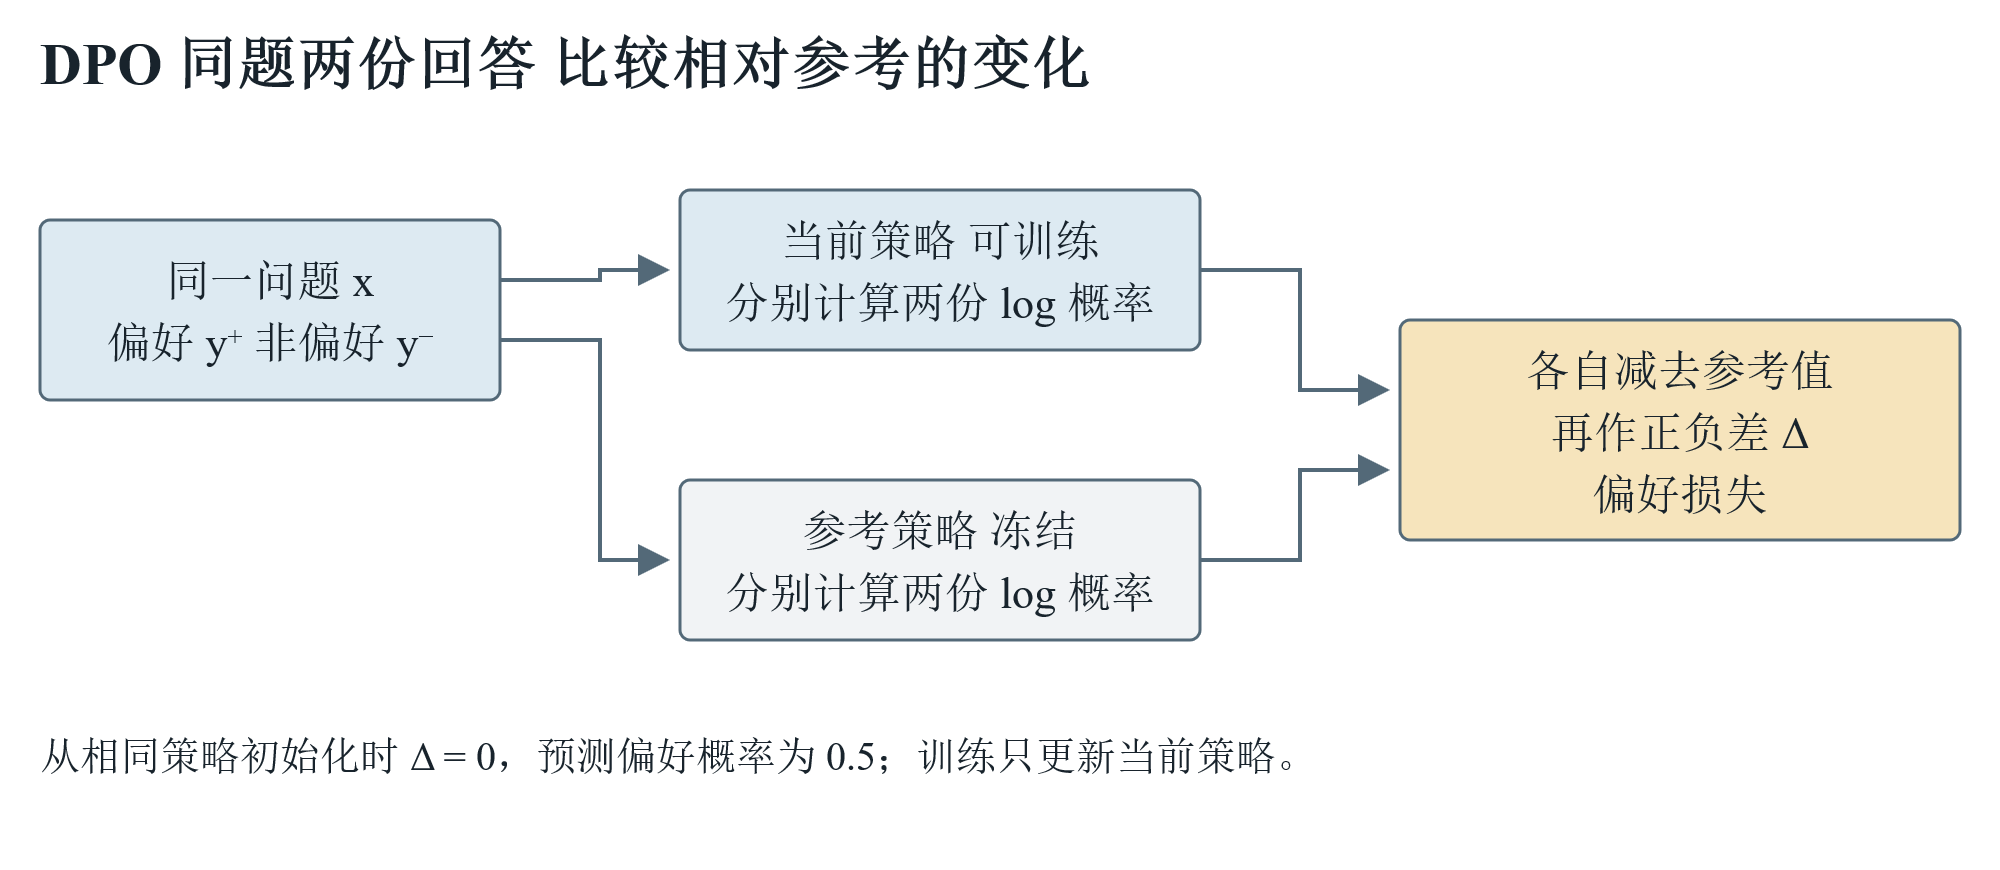
\includegraphics[width=\linewidth]{assets/media/image16.png}
    \caption{DPO 的比较对象。参考策略参与计算但不随本次损失更新；梯度只更新当前策略。离线数据是否覆盖当前行为，需要在下一节另行检查。}
    \label{fig:DPO比较对象}
\end{figure}

进一步看单对样本的梯度，就能看到两份回答如何共同提供训练信号。参考模型保持冻结，有
\[
\nabla_\theta\ell_\theta
=-\beta\sigma(-\beta\Delta_\theta)
\left[\nabla_\theta\log\pi_\theta(y^+\mid x)
-\nabla_\theta\log\pi_\theta(y^-\mid x)\right].
\]
梯度下降要减去这个梯度，因此更新方向包含提高偏好回答对数概率的方向，以及降低偏恶回答对数概率的方向。前面的权重会在模型尚未符合这对偏好时较大，在模型已经明显拉开差距时较小。两份回答共用网络参数，实际不能保证每一步都让前者的绝对概率上升、后者的绝对概率下降；目标直接约束的是它们相对参考模型的概率比。

回答的对数概率又是逐 token 对数概率之和：
\[
\log\pi_\theta(y\mid x)
=\sum_{t=1}^{|y|}\log\pi_\theta(y_t\mid x,y_{<t}).
\]
因此，偏好信号最终通过这些 token 的对数概率反向传播到模型权重。许多偏好对一起调整生成分布，让类似输入下的行为更符合标注偏好。能否推广到新问题，仍取决于数据覆盖与模型泛化；序列级标签也不会自动指出偏恶回答究竟错在哪个 token。

这里用的是回答序列的概率，实际通过 token log probability 加总计算，通常不把提示文本（prompt）对应的 token 计入回答概率。长短答案、截断、补齐掩码（padding mask）和模板仍会影响结果。它与 SFT 一样可以 teacher forcing 计算给定回答的概率，但损失还比较正负回答和与参考模型的偏离程度，并非等价于 SFT。

我们把四次概率计算画在图 \ref{fig:DPO比较对象}：两份回答分别经过当前策略与冻结参考策略。先减参考，再比较正负，才能得到前面定义的 Δ。

我们用一个小例子观察参考的作用。假如训练策略从参考初始化，最初每份回答的对数概率比都为零，Δ 也为零，对这对样本预测偏好概率为 0.5。训练再根据标签拉开相对差异。若标签总偏爱长答案，模型也可能学到长度捷径。

DPO 的理论联系建立在偏好建模与理想化优化条件上。有限数据、受限模型族和分布外输入，会使实际行为偏离理想。我们获得的是一种直接优化方式，仍然需要训练和独立评估。

\textbf{实践}~用 DPO 方法训练一个小模型，观察它在训练集和独立评估集上的行为，比如有一些开源项目训练原始模型为网店客服的语言风格。

\textbf{本节相关资料}
\begin{enumerate}
    \item Rafailov 等，2023，\href{https://arxiv.org/abs/2305.18290}{Direct Preference Optimization Your Language Model is Secretly a Reward Model}。\textbf{提出 DPO 方法的论文}。阅读重点：从最优策略关系反解奖励，以及为什么归一化项在偏好比较中抵消。
    \item Azar 等，2023，\href{https://arxiv.org/abs/2310.12036}{A General Theoretical Paradigm to Understand Learning from Human Preferences} 。阅读重点：偏好建模和优化目标的假设怎样影响方法选择。
\end{enumerate}

\section{离线与在线偏好优化 数据如何跟上策略}\label{离线与在线偏好优化 数据如何跟上策略}

我们用同一份偏好集做了许多轮 DPO。训练集的偏好分类越来越容易，实际对话却出现一类新错误：模型在较长的解释中反复自我肯定。旧偏好数据里没有这种回答，我们也从未评价过它。此时，问题从``如何拟合标签''转为``标签覆盖了谁的行为''。

离线偏好优化把已有回答当作固定训练材料。我们不需要在每个优化步骤在线生成，成本容易控制，数据也便于审核。可当策略（也就是模型行为）发送明显变化，静态样本未必覆盖新模型常生成的轨迹。

我们可以周期性让当前模型生成新候选，再标偏好、再优化。这是在线或迭代偏好优化的一种思路。它把反馈追到学生的新行为上，但也增加采样、评审与版本管理成本。一次收集、多轮训练与持续重采样之间存在很多中间方案，不是非此即彼。

DPO 存在许多变体方法，我们继续用三个问题定位：信号是什么，数据由谁产生，更新依赖哪些组件。恒等偏好优化（Identity Preference Optimization，IPO）研究另一类偏好目标；卡尼曼与特沃斯基优化（Kahneman--Tversky Optimization，KTO）可以使用好坏标签而不要求每条都是成对偏好；简单偏好优化（Simple Preference Optimization，SimPO）以平均序列对数概率构造无参考奖励；优势比偏好优化（Odds Ratio Preference Optimization，ORPO）把监督学习与偏好约束结合，省去独立参考模型。知道这些差别，就能理解它们各自减少了什么成本，而不急着背公式清单。

我们会先选实现清楚、数据适配的方法建立基线。当独立评估显示静态数据覆盖不足，再引入迭代收集。这个顺序使每一次复杂度增加都对应已观察到的需求。

需要注意的是，与 LoRA 一样，工业领域基础模型团队为了确保训练框架简单可靠，通常不会支持太多分支功能，因此可能也不支持 DPO 训练，因为通常可以通过强化学习解决相同问题。

\textbf{本节相关资料}
\begin{enumerate}
    \item Azar 等，2023，\href{https://arxiv.org/abs/2310.12036}{A General Theoretical Paradigm to Understand Learning from Human Preferences}，包含 IPO 。阅读重点：为何要重新检查偏好目标。
    \item Ethayarajh 等，2024，\href{https://arxiv.org/abs/2402.01306}{KTO Model Alignment as Prospect Theoretic Optimization} 。阅读重点：不成对的好坏标签怎样提供信号。
    \item Meng 等，2024，\href{https://arxiv.org/abs/2405.14734}{SimPO Simple Preference Optimization with a Reference-Free Reward} 。阅读重点：参考模型与长度处理的改变。延伸比较 ORPO：\href{https://arxiv.org/abs/2403.07691}{{原文链接}} 。
\end{enumerate}

\section{RL 泛化诊断 训练涨分而验证不涨}\label{RL 泛化诊断 训练涨分而验证不涨}

我们完成一轮 RL，训练奖励从教学案例中的 0.35 升到 0.70，验证集答案正确率却几乎不动意味着我们必须立即开始检查。

``训练涨''可能指在线生成轨迹（rollout）的奖励，也可能指固定训练题的独立评估；``验证不涨''可能指最终答案正确率，也可能指人工偏好。若前者是代理 RM 分数，后者是真实任务质量，两个指标原本就不等价。我们必须在固定训练题和验证题上，都用同一套解码预算与独立评分重评一次，把测量差异先拿掉。通常来说，我们需要同时观察 reward 曲线、rollout 准确率曲线和验证集准确率曲线。

第一种可能是记住了题目或模板。我们按原始题族切分，测试换数值、换叙述、换组合方式。若只在见过的表述上变好，继续增加同类重复题可能让曲线更漂亮，却不能支持迁移。我们应补充机制相同但表面不同的训练覆盖，并保留真正未参与开发的测试题。

第二种可能是奖励被钻空子，称为奖励黑客（reward hack）。小助把``因此答案正确''写得更频繁，RM 更喜欢，独立验证器却看不到改善。我们检查高奖励失败样本，尤其看奖励提升最大的部分。必要时修评分规范、增加反例、改验证器，再从合理检查点重训。\textbf{需要注意的是，reward hack 已经成为目前 RL 训练的最根本问题之一，理论上说，如果能根除 reward hack，那么我们可以训练出任何想要的模型能力。} Reward hack 存在许多形式，有的简单有的复杂，复杂的非常难识别和抑制，我们也许可以调用一个超强外部模型来判别，但是强化学习需要大量 rollout，大量强模型的判别的成本极高，人工专家判别则效率过低。目前，reward hack 已经成为最难解决的问题之一，这也吸引了大量研究者投入到 reward hack 的研究中。

第三种可能是训练与验证题目分布不同，就是题目之间差距太大。训练主要是一两步代数，验证集更多是长条件、多步组合。训练收益可能真实，但局限于训练集已覆盖的能力区域。我们按知识点和难度分桶，看哪些桶有迁移，再决定补数据、安排课程学习或调整目标任务。

第四种可能是评估噪声或预算变化。小评估集、随机采样、答案解析错误，都能掩盖变化。我们报告题目数和重复次数，对同一题做成对比较，必要时估计置信区间。若新模型用了更长输出或更多采样，还需观察质量与 token 成本的关系。

我们可以把证据整理为一个紧凑矩阵，再选下一步实验。

\begin{longtable}[]{@{}
  >{\raggedright\arraybackslash}p{(\linewidth - 4\tabcolsep) * \real{0.2985}}
  >{\raggedright\arraybackslash}p{(\linewidth - 4\tabcolsep) * \real{0.2985}}
  >{\raggedright\arraybackslash}p{(\linewidth - 4\tabcolsep) * \real{0.4030}}@{}}
\toprule\noalign{}
\begin{minipage}[b]{\linewidth}\raggedright
\textbf{观察}
\end{minipage} & \begin{minipage}[b]{\linewidth}\raggedright
\textbf{优先假设}
\end{minipage} & \begin{minipage}[b]{\linewidth}\raggedright
\textbf{下一步检查}
\end{minipage} \\
\midrule\noalign{}
\endhead
\bottomrule\noalign{}
\endlastfoot
训练 RM 涨 独立正确率不涨 & 奖励偏离真实目标 & 人工审查高奖励失败样本 \\
固定训练题涨 未见题不涨 & 记忆或覆盖不足 & 按题族和难度分桶重评 \\
答案更长 得分差异不稳定 & 预算或测量混淆 & 固定 token 与采样预算 \\
一个题型涨 另一个题型降 & 收益不均或能力干扰 & 分项指标与旧能力回归测试 \\
\end{longtable}

\textbf{本节相关资料}
\begin{enumerate}
    \item Gao 等，2022，\href{https://arxiv.org/abs/2210.10760}{Scaling Laws for Reward Model Overoptimization} 。阅读重点：怎样分别衡量代理目标与更可信的目标。
    \item Srivastava 等，2022，\href{https://arxiv.org/abs/2206.04615}{Beyond the Imitation Game Quantifying and extrapolating the capabilities of language models} 。阅读重点：任务多样性为何影响我们对能力的判断。
\end{enumerate}

\section{RL 训练诊断 从数据与判题检查到补回 SFT}\label{RL 训练诊断 从数据与判题检查到补回 SFT}

另一轮实验中，小助的训练奖励几乎是一条直线。我们先做一次很小的链路检查：确认官方样例或简单题能运行、参数确实更新、采样端加载了新权重、奖励方向没有写反。使用经过验证的成熟训练基础设施（infrastructure，常简称 infra）\footnote{推荐了解 Slime 和 VeRL 这两种框架，都是工业界最常用的强化学习基础设施，也推荐读者自行基于这些 infra 实践。这些 infra 本身的优化也是现代人工智能领域的重要研究课题。}，并确认关键配置后，我们把主要排查精力转向题目难度、参考答案与判题器。这是当前实验的排查顺序，不是对所有框架故障率的统计结论；有明确异常日志时，仍应沿证据检查实现。

\textbf{先看数据是否处在可学习的难度区间}~我们固定采样预算，对每题生成一组回答，查看每题成功率与同分组比例。如果绝大多数题都远超小助当前能力，组内反复全错，GRPO 就缺少有用的相对奖励信号。我们先排除错答案和误判，再适当降低题目难度、补充中间难度题或拆分子任务。全对题也不能不看覆盖需求就全部删除；目标是让当前策略有机会产生可以比较的尝试。最终纳入强化学习训练的样本，通常是正确率不那么高，但是能够采样到过程和答案都正确轨迹的题目。

\textbf{造数据时就交叉核验答案}~我们不把一个强模型生成的答案直接当作标准答案。先让多个强模型独立解题，尽量不向它们展示候选标准答案，避免互相照抄或被同一答案锚定；再把最终答案按约定格式归一化，比较是否一致。有分歧的题先复核、重写或剔除。模型之间也可能共享错误，所以一致只是筛选信号；能用计算、执行、符号检验或原始资料确认的题，应继续核验，并抽样人工检查一致通过的样本。

我们把用于自动判分的最终答案设计得简短清晰，例如一个词语、一个数值或一个短语，同时保存可核查的解题依据。数值题预先规定单位、精度与容差；词语和短语题规定合理的别名、大小写与等价表达。这里约束的是最终答案与判分接口，推理过程仍可按任务需要保留。题目本身也要避免条件缺失、多解却只登记一个答案等问题。

\textbf{把判题器当作需要验收的组件}~我们用已知正确、已知错误及边界样本测试判题规则。例如``5''\,``5.0''\,``a＝5''是否应当等价，要由这道题的答案规范决定；``5 米''不能在量纲不符时仅因含有数字 5 就得分。我们检查答案抽取、等价判断、单位、超时和空输出，再抽样复核真实 rollout。假阴性样本会让有效尝试拿不到奖励，假阳性样本则可能让模型学会利用判题漏洞。

\textbf{优先构造短答案题，谨慎使用选择题}~选择题让模型可以通过猜测、排除或选项中的表面线索得分，而不必完成我们希望训练的求解。因此，在能够可靠判分时，我们优先让小助直接给出词语、数值或短语，而不是把训练题默认做成四选一。猜中本身不等于奖励投机，但持续利用选项位置、措辞或解析漏洞，会使奖励与实际求解能力脱离。

如果任务必须使用单选题，我们可以把候选数扩展到 10 项，条件允许时再试 20 项，并保证干扰项有意义、题目仍有唯一正确答案。在完全均匀盲猜且只有一个正确选项时，命中率分别是 10\% 和 5\%；这不是实际模型的猜测率保证。无效干扰项容易被排除，增加选项还会增加输入长度与阅读难度，因此要比较这些变化后的真实收益。

在造题目时，我们可以为每次 rollout 独立打乱选项顺序，并同时重建显示标签与正确答案映射。稳定保存每个选项的内容标识、排列和随机种子，判题时先把模型选择映射回实际内容，再与标准答案比较。若只打乱选项却沿用原来的字母答案，反而会制造错误奖励；``以上皆是''等依赖位置的表述也须先改写。

排查完数据与判题，再看温度、生成长度、KL 约束、学习率、优势与裁剪：输出是否过度重复，是否被截断，更新是否过弱？我们一次改一个因素。若干净题目和可靠判题都已确认，而模型在可接受预算内仍反复缺少关键步骤，再用经审核的针对性 SFT 示范建立起点。补完以后，先检验留出题，再观察是否出现更多有效尝试与组内差异，最后重启 RL。

我们在示范与反馈之间按证据往返。成熟链路做简短确认，数据难度、答案与判题做重点复核；补 SFT 的依据通常是 rollout 尝试全部失败，都出现关键过程或者结果错误。

还有一点需要了解的是，强化学习仅仅训练少量专用数据也几乎不会造成灾难性遗忘，这与 SFT 截然不同。

\textbf{本节相关资料}
\begin{enumerate}
    \item Pezeshkpour 与 Hruschka，2023，\href{https://arxiv.org/abs/2308.11483}{Large Language Models Sensitivity to The Order of Options in Multiple-Choice Questions} 。阅读重点：选项排列如何影响测量；正文中的 10 或 20 项与逐次打乱是需要在具体任务中验证的工程建议，并非该论文给出的通用最优配置。
\end{enumerate}